\section{Volume Estimation}
\label{volume estimation}
\label{testing:vol est} %delete this and die 
This section details the testing of the volume estimation algorithm as well as touching on the testing of the circumference estimation.

\subsection{Determining the Transform Constant Using Volume}
\label{determining the transform constant}
Initially, the transform constant was to be calculated in terms of volume. The approach planned was for many people to be scanned and their minimum bounding box calculated two ways. Firstly the box would calculated using the PARSE toolkit to give the box's volume in PCS. Secondly, the volume of the box would be calculated in RWS by measuring the height, width and breadth of the person. These figures would then be divided to determine the transform constant as in equation \ref{testing: calculating the transform constant}.\\

\begin{equation}
\frac{Volume_{RWS}}{Volume_{PCS}} = Transform Constant
\label{testing: calculating the transform constant}
\end{equation}\\

However, delays in the stitching algorithm for the four individual scans were holding up the determination of the transform constant via this method and therefore the testing of the overall volume estimation. As such, a different approach was taken. 

\subsection{Determining the Transform Constant Using Height}
\label{determining the transform constant using height}
Instead of measuring a bounding box two ways, the transform constant would be determined in terms of height, as in equation \ref{testing: calculating the transform constant using height}. This method would only required un-stitched scans. Using height resulted in the need to cube the constant to transform 3-dimensional quantities such as volume.\\

\begin{equation}
\frac{Height_{RWS}}{Height_{PCS}} = Transform Constant
\label{testing: calculating the transform constant using height}
\end{equation}

In order to determine the transform constant, twenty two subjects were scanned and their height measured in both point cloud units (PCU) using the tool kit and in meters using a tape measure. Using the data in Table \ref{testing: table of data used to calculate the transform constant}, a transform constant was calculated for each subject.\\

\begin{table}[!htb]
\begin{center}
  \begin{tabular}{| l | p{3cm} | p{2cm} | p{2cm} |}
    \hline
    Person & $Height_{RWS}$ ($m$) & $Height_{PCS}$ & Transform Constant \\ \hline
    Adams & 1.88 & 2.29 & 0.82\\ \hline
    Alissa & 1.86 & 2.27 & 0.82 \\ \hline
    Anonymous 1 & 1.82 & 2.28 & 0.80\\ \hline
    Anonymous 2 & 1.76 & 2.24 & 0.78\\ \hline
    Archbold & 1.82 & 2.26 & 0.80\\ \hline
    Bradbury & 1.72 & 2.11 & 0.82\\ \hline
    Corbett & 1.94 & 2.29 & 0.85\\ \hline
    Fletcher & 1.80 & 2.25 & 0.80\\ \hline
    Getley & 1.85 & 2.26 & 0.82\\ \hline
    Griffiths & 1.84 & 2.27 & 0.81\\ \hline
    Janssens & 1.85 & 2.26 & 0.82\\ \hline
    Jin	& 1.81 & 2.24 & 0.81\\ \hline
    Kozlowska & 1.64 & 2.09 & 0.78\\ \hline
    Marshall & 1.73 & 2.12 & 0.81\\ \hline
    McCutcheon & 1.88 & 2.29 & 0.82\\ \hline
    Mermet & 1.70 & 2.11 & 0.80\\ \hline
    Page & 1.82 & 2.28 & 0.80\\ \hline
    Papaconstantinou & 1.69 & 2.10 & 0.81\\ \hline
    Richardson & 1.58 & 2.00 & 0.79\\ \hline
    Rayment & 1.92 & 2.29 & 0.84\\ \hline
    Taplin & 1.62 & 2.08 & 0.78\\ \hline
    Wicks &1.90 & 2.29 & 0.83\\ \hline
  \end{tabular}
\end{center}
\caption{Table of data used to calculate the Transform Constant (to two decimal places)}
\label{testing: table of data used to calculate the transform constant}
\end{table}

From these twenty two transform constants, an average transform constant was calculated to be 0.81 (to two decimal places). 

\subsection{Height Estimation}
\label{height estimation}
Using an average transform constant is a \emph{one size fits all} approach and will introduce errors into the height estimation. These errors are expected to be related to the distance a subject is from the average height and was quantified by predicting the height of a subject as per equation \ref{predicting real world height}.\\

\begin{equation}
Height_{PCS} * Average Transform Constant = Height_{RWS}
\label{predicting real world height}
\end{equation}

Table \ref{errors in determining a subjects height} shows for each subject, their absolute distance from the average sample height (ADFAH), the predicted height and the error in this prediction when compared to the subjects actual height in meters.\\ 

\begin{table}[!htb]
\begin{center}
  \begin{tabular}{| l | p{2.5cm} | p{2cm} | p{2cm} |}
    \hline
    Person & ADFAH (m) & Predicted Height (m) & Error (\%) \\ \hline
    Alissa & 0.07 & 1.84 & 1.16\\ \hline
    Anonymous 1 & 0.03 & 1.85 & 1.60\\ \hline
    Anonymous 2	& 0.03 & 1.82 & 3.14\\ \hline
    Archbold & 0.03 & 1.83 & 0.61\\ \hline
    Bradbury & 0.07 & 1.71 & 0.82\\ \hline
    Corbett	& 0.15 & 1.85 & 4.80\\ \hline
    Getley & 0.06 & 1.83 & 0.98\\ \hline
    Fletcher & 0.01 & 1.82 & 1.18\\ \hline
    Griffiths & 0.05 & 1.83 & 0.28\\ \hline
    Janssens & 0.06 & 1.83 & 0.98\\ \hline
    Jin & 0.02 & 1.82 & 0.39\\ \hline
    Kozlowska & 0.15 & 1.69 & 3.10\\ \hline
    Marshall & 0.06 & 1.72 & 0.63\\ \hline
    McCutcheon & 0.09 & 1.85 & 1.56\\ \hline
    Mermet & 0.09 & 1.71 & 0.61\\ \hline
    Page & 0.03 & 1.85 & 1.61\\ \hline
    Adams & 0.09 & 1.85 & 1.38\\ \hline
    Richardson & 0.21 & 1.62 & 2.34\\ \hline
    Papaconstantinou & 0.10 & 1.70 & 0.46\\ \hline
    Rayment & 0.13 & 1.85 & 3.75\\ \hline
    Taplin & 0.17 & 1.69 & 3.89\\ \hline
    Wicks & 0.11 & 1.85 & 2.58\\ \hline
  \end{tabular}
\end{center}
\caption{Errors in determining a subjects height}
\label{errors in determining a subjects height}
\end{table}

It was suspected that error was related to the subjects absolute distance from average height. Therefore, error has been plotted against this distance in Figure \ref{distance vs error}.\\

\begin{figure}[!htb]
\begin{center}
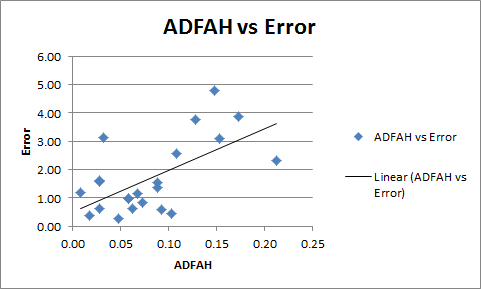
\includegraphics[scale=0.8]{images/distvserror} 
\end{center}
\caption{Distance vs Error}
\label{distance vs error}
\end{figure} 

ADFAH and error have a Pearson product-moment correlation coefficient of 0.61, suggesting a medium strength correlation \cite{cohen88,buda2011} between the two quantities. This suggests the averaging approach to determining the transform constant has the limitation that a subject must be average height, in terms of the sample used to determine the TC, in order for the most accurate result.\\

The errors in predicted height from the test subjects can be used to determine a approximate error range for estimating height of a subject between 1.58m and 1.94m. This range is the taken from the real world heights in Figure \ref{testing: table of data used to calculate the transform constant}. The average as well as the standard deviation error were determined as in Table \ref{average and standard deviation of error}. From these values, the height estimation could be said to have an accuracy of $\pm$4.25\%. This value is based on the fact that height is often assumed to be normally distributed \cite{chali1995} and ~95\% of the values of a normal distribution typically lie within 2 standard deviations of the mean value \cite{pukelsheim1994}.\\

\begin{table}[!htb]
\begin{center}
  \begin{tabular}{| l | l |}
    \hline
    Average Error (\%) & 1.72\\ \hline
    Standard Deviation of Error & 1.26\\ \hline
  \end{tabular}
\end{center}
\caption{Average and standard deviation of error}
\label{average and standard deviation of error}
\end{table}

The above determination of the transform constant allowed for the volume estimation to be tested on scans of a sufficient quality that the initial Bounding Box method of stitching aligned them near perfectly, as was the case for the Corbett data set, see Figure \ref{fig:the_corbett_data_set}. This testing is elaborated on in Section \ref{testing: volume calculation}.\\

\subsection{Errors in Height Measurement}
Calculating the transform constant in the manner described in Figure \ref{testing: calculating the transform constant using height} is not without drawbacks. The main drawback is that the real world measurements must be calculated by hand, using a tape measure. Such a process is inherently error prone, as highlighted in Section \ref{spec:motivation}. However it was hoped that, by taking as large a sample as possible and averaging the transform constants, such errors would be eliminated or at least minimised.\\

\subsection{Consistency of Height Measurement}
Whilst the one time error of the system is important to quantify, the consistency is also of note. To quantify this, the Corbett subject was repeatedly scanned the height of the subject measure. Using the data from Figure \ref{testing: table of data used to calculate the transform constant} as the gold standard, the average error over twenty scans was 2\% and the maximum error of 4\%, based on the standard deviation \cite{pukelsheim1994}.\\

\subsection{Plane Retrieval}
This section details the testing of the method to retrieve a plane of points, all at a similar height, from a point cloud was tested by outputting the retrieved points x and z co-ordinates to a .csv file and plotting them using Excel. Using Excel meant that the retrieval method could be tested outside the visualisation, which was at this stage untested. For testing purposes we took a slice from the approximate middle, height wise, of the Wilkinson data set, visualised in Figure \ref{fig:the wilkinson data set, visualised with the bounding box stitching method}.\\

\begin{figure}[!htb]
\begin{center}
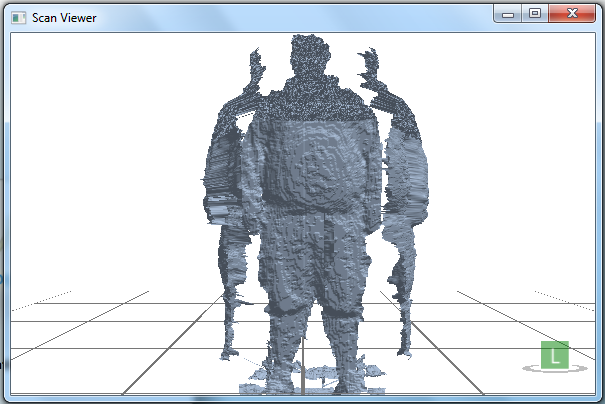
\includegraphics[scale=0.4]{images/wilko1} 
\end{center}
\caption{The Wilkinson data set, visualised with the Bounding Box stitching method.}
\label{fig:the wilkinson data set, visualised with the bounding box stitching method}
\end{figure}

Through Excel, the group was able to determine the middle plane from the Wilkinson data set was being correctly retrieved, see Figure \ref{fig:the middle plane of the Wilkinson data set, visualised in excel.}. Also, the Excel visualisation was a gold standard that informed the verification of the PARSE toolkit visualisation, see Figure \ref{fig:The middle plane of the wilkinson data set, visualised in the parse toolkit.}.\\ 

\begin{figure}[!htb]
\begin{center}
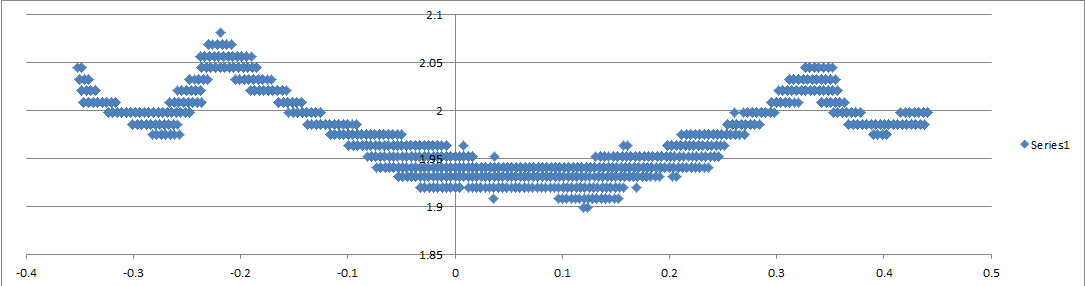
\includegraphics[scale=0.4]{images/wilko2} 
\end{center}
\caption{The middle plane of the Wilkinson data set, visualised in Excel.}
\label{fig:the middle plane of the Wilkinson data set, visualised in excel.}
\end{figure}

\begin{figure}[!htb]
\begin{center}
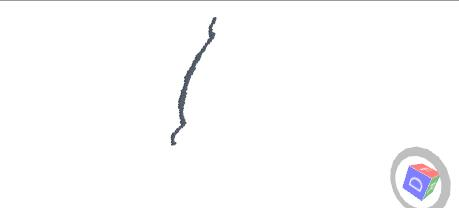
\includegraphics[scale=0.4]{images/wilko3} 
\end{center}
\caption{The middle plane of the Wilkinson data set, visualised in the PARSE toolkit.}
\label{fig:The middle plane of the wilkinson data set, visualised in the parse toolkit.}
\end{figure}

\subsection{Using a Bath to Calculate Gold Standards for Volume}
In order to test the accuracy of the toolkit's volume estimation, a gold standard would be required. This volume was achieved by calculating the volume of water a person displaced \cite{katch1967}. This was achieved by filling the bath to a level and marking the level. The subject then sits in the bath, fully submerged, and a new mark made. The person then exits the bath after all the water has dripped off their body. Using a jug \cite{beynon1989} of known volume, the water level is increased until the level meets the second mark. From the number of jugs used, a gold standard volume can be determined. Table \ref{the volume of group members} shows these gold standards. Whilst they are being treated as true values, in reality it is unlikely they are. Reasons for this will be discussed in later in Section \ref{errors in volume measurement}.\\

\begin{table}[!htb]
\begin{center}
  \begin{tabular}{| l | l |}
    \hline
    Name (\%) & Volume ($m^3$)\\ \hline
    Bernard & 0.058\\ \hline
    Nathan & 0.062\\ \hline
    Greg & 0.064\\ \hline
  \end{tabular}
\end{center}
\caption{The volume of group members}
\label{the volume of group members}
\end{table}

\subsection{Volume Calculation}
\label{testing: volume calculation}
From the values in Table \ref{average and standard deviation of error}, hypothetical average error and the corresponding standard deviation can be approximated by cubing those values. Table \ref{hypothetical average and standard deviation of error} shows these hypothetical values. Hence, the volume estimation could be said to have an accuracy of between $\pm$1.06\% and $\pm$9.12\%. The Bod Pod has been shown to have similar error ratings \cite{fields2001,collins2004}.\\

\begin{table}[!htb]
\begin{center}
  \begin{tabular}{| l | l |}
    \hline
    Average Error (\%) & 5.09\\ \hline
    Standard Deviation of Error & 2.01\\ \hline
  \end{tabular}
\end{center}
\caption{Hypothetical average and standard deviation of error of volume estimation}
\label{hypothetical average and standard deviation of error}
\end{table}

Using the toolkit, the volume of group members were calculated and are displayed in Table \ref{the volume of group members measured by the tool kit}. The volume of the Corbett subject was averaged over four scans.\\

\begin{table}[!htb]
\begin{center}
  \begin{tabular}{| l | l | l |}
    \hline
    Name (\%) & Volume ($m^3$) & Error (\%)\\ \hline
    Bernard & 0.07
 & 20.69\\ \hline
    Nathan & 0.075 & 20.97\\ \hline
    Greg & 0.0816 & 27.50\\ \hline
  \end{tabular}
\end{center}
\caption{The volume of group members measured by the tool kit}
\label{the volume of group members measured by the tool kit}
\end{table}

From Table \ref{the volume of group members measured by the tool kit}, the volume estimation could be said to have an average error measure of 23.05\%.

\subsection{Errors in Volume Measurement}
\label{errors in volume measurement}
Clothing can artificially inflate a subjects volume when scanned \cite{shafer2008}. It must be noted that the gold standard for a subject was determined whilst the subject was in a state of undress, whereas the scan were taken in a public work area hence clothes were worn, this may be the reason for the volume estimation consistently overestimating by approximately 20\%. A better measure to compare volumes and comment on the estimations accuracy may be ``the Bernard", defined in \ref{the bernard defined}. Using the Bernard, the gold standard volumes and the volumes calculated by the toolkit can be expressed as in Table \ref{The volume of group members in bernards}.\\

\begin{figure}[!htb]
\begin{center}
  \textit{Definition: 1 Bernard is the volume of Bernard Sexton, as calculated by the method provided by the context.}
\end{center}
\caption{The Bernard defined}
\label{the bernard defined}
\end{figure}

\begin{table}[!htb]
\begin{center}
  \begin{tabular}{| l | p{4cm} | p{3cm} | p{2cm} |}
    \hline
    Name (\%) & Gold Standard Volume (Bernards) & Toolkit Volume (Bernards) & Error (\%)\\ \hline
    Bernard & 1.00 & 1.00 & 0.00\\ \hline
    Nathan & 1.07 & 1.07 & 0.23\\ \hline
    Greg & 1.10 & 1.17 & 5.64\\ \hline
  \end{tabular}
\end{center}
\caption{The volume of group members in Bernards}
\label{The volume of group members in bernards}
\end{table}

Hence, the ratios of volumes between the three group members are fairly consistent when measured with both the gold standard bath tub and the toolkit, with an average error of 1.96\%. The majority of this error is associated with the Corbett subject who, as shown in Section \ref{height estimation}, is far away from the average height, so 4\% of the 5.64\% may be caused by his above average height. Excluding this height caused error would bring the average error of the ratios down to 0.62\%, but more test subjects are needed before any real conclusions can be made.\\

When calculating the gold standards factors such as water dripping, skin absorption and surface evaporation can all introduce errors. If the subject is not completely dry when they exit the bath the volume will be marginally overestimated. The skin of the subject may also absorb some of the water and whilst the measurements are being taken some of the water may evaporate again causing the volume to be overestimated. The jugs used to measure the quantity of water returned to the bath only give approximate measurements \cite{ikea,pyrex}. The refilling of the bath via these jugs is also vulnerable to parallax errors. Noisy scan data will also introduce random error into the estimations.\\

\subsection{Circumference Measurement and Errors}
\label{errors in circumference measurement}
In order to test the circumference measurements, the Corbett subject's circumference was measured with a tape measure at 0.49m, 0.97m and 1.46m corresponding to planes 45, 30 and 15. The results are reproduced in Table \ref{the circumference of the Corbett subject measured with the tool kit} and were treated as gold standards. The tool kit was then used to measures these circumferences using the same four scans as in Table \ref{the volume of group members measured by the tool kit}. The results are reproduced in Table \ref{the circumference of the Corbett subject measured with the tool kit}.\\

\begin{table}[!htb]
\begin{center}
  \begin{tabular}{| l | p{3cm} | p{3cm} | p{2cm} |}
    \hline
    Height (m) & Gold Standard Circumference (m) & Average Circumference (m) & Error (\%)\\ \hline
    0.49 & 0.62 & 0.56 & 10.14\\ \hline
    0.97 & 0.88 & 0.87 & 1.60\\ \hline
    1.46 & 1.06 & 0.91 & 14.41\\ \hline
  \end{tabular}
\end{center}
\caption{The circumference of the Corbett subject measured with the tool kit.}
\label{the circumference of the Corbett subject measured with the tool kit}
\end{table}

As previously mentioned, 4\% of this error may be caused by the Corbett subject being far away from the average height. As such, the circumference estimation could be said to be accurate to within $\pm$10\%. Clothing can increase the error on a circumference measure, a t-shirt sleeve suitable positioned can add 10cm to the circumference value so the true error rating may be less than this.\\

\section{The Breast Problem}
\label{testing:the breast problem}
\emph{The Breast Problem}  is an umbrella term coined to describe the many problems caused by the anatomical differences between the genders. An example of such a problem is the degree of accuracy when stitching with the Bounding Box method.\\

Another example is the errors when measuring circumferences caused by bras. It has already been shown that clothing can have a big impact on the measurement of circumferences in Section \ref{errors in circumference measurement}. If, for example, a measurement is needed at about breast height, the type of bra the patient is wearing may affect the data returned. An underwired bra may increase the circumference at this height or expose a previously occluded area of ``underboob". This issue has been previously noted by those determining the accuracy of the BOD POD \cite{shafer2008}.\\